\documentclass[tikz,border=10pt]{standalone}
\usepackage{tikz}

% ---------- palette ----------
\definecolor{wallColor}{RGB}{243,225,196}
\definecolor{wallColorDark}{RGB}{214,192,157}
\definecolor{floorColor}{RGB}{176,130,94}
\definecolor{floorColorDark}{RGB}{150,108,76}
\definecolor{baseboardColor}{RGB}{112,78,54}

\definecolor{windowFrameColor}{RGB}{90,60,42}
\definecolor{nightSky}{RGB}{30,40,74}
\definecolor{moonColor}{RGB}{250,244,214}
\definecolor{rodColor}{RGB}{80,54,38}
\definecolor{curtainColor}{RGB}{176,60,66}
\definecolor{curtainColorDark}{RGB}{140,42,50}
\definecolor{curtainHighlight}{RGB}{202,96,98}

\definecolor{clockFrameColor}{RGB}{90,60,42}
\definecolor{clockFaceColor}{RGB}{250,244,224}

\definecolor{rugColor}{RGB}{170,70,58}
\definecolor{rugColorDark}{RGB}{140,52,44}
\definecolor{rugColorLight}{RGB}{206,120,96}

\definecolor{lampPoleColor}{RGB}{70,55,45}
\definecolor{lampShadeColor}{RGB}{250,225,168}
\definecolor{lampShadeDark}{RGB}{221,188,128}
\definecolor{lampGlowColor}{RGB}{255,238,190}

\definecolor{tableColor}{RGB}{120,82,55}
\definecolor{tableColorDark}{RGB}{96,64,42}

\definecolor{tvStandColor}{RGB}{96,64,42}
\definecolor{tvFrameColor}{RGB}{38,38,42}
\definecolor{tvScreenColor}{RGB}{178,212,226}
\definecolor{tvScreenDark}{RGB}{140,182,206}
\definecolor{tvGlowColor}{RGB}{192,222,233}
\definecolor{tvSunColor}{RGB}{240,168,104}

\definecolor{chairColor}{RGB}{88,128,118}
\definecolor{chairColorDark}{RGB}{66,100,92}
\definecolor{chairColorLight}{RGB}{114,154,142}

\definecolor{skinColor}{RGB}{236,201,177}
\definecolor{skinColorShadow}{RGB}{212,174,148}
\definecolor{hairColor}{RGB}{227,227,223}
\definecolor{hairColorDark}{RGB}{198,198,193}

\definecolor{cardiganColor}{RGB}{168,78,66}
\definecolor{cardiganColorDark}{RGB}{136,58,50}

\definecolor{blanketColor}{RGB}{214,176,108}
\definecolor{blanketColorDark}{RGB}{186,146,82}

\definecolor{slipperColor}{RGB}{150,60,58}
\definecolor{glassesColor}{RGB}{60,50,45}
\definecolor{caneColor}{RGB}{112,82,56}
\definecolor{potColor}{RGB}{150,90,60}
\definecolor{leafColor}{RGB}{96,134,74}

\begin{document}
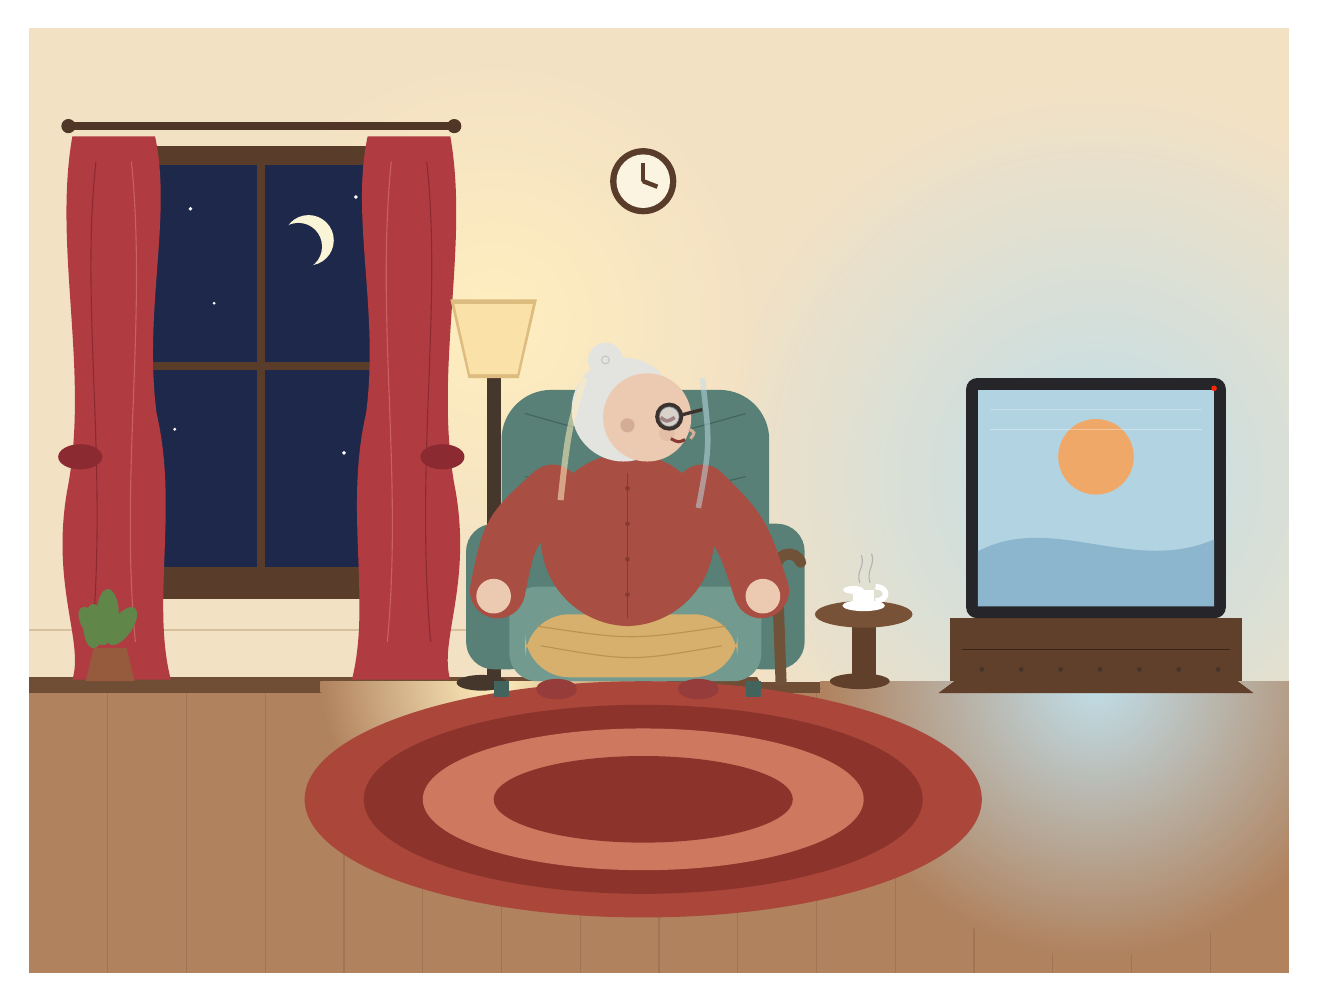
\begin{tikzpicture}

  % ============ background: wall + floor ============
  \fill[wallColor] (0,3.7) rectangle (16,12);
  \fill[floorColor] (0,0) rectangle (16,3.7);
  \draw[wallColorDark, line width=1pt] (0,4.35) -- (16,4.35);
  \foreach \x in {1,...,15}{
    \draw[floorColorDark, thin, opacity=0.55] (\x,0) -- (\x,3.7);
  }
  \fill[baseboardColor] (0,3.55) rectangle (16,3.75);

  % ============ ambient glow: TV (right side, cool light) ============
  \begin{scope}
    \clip (0,3.7) rectangle (16,12);
    \shade[shading=radial, inner color=tvGlowColor, outer color=wallColor]
      (13.55,6.3) circle (5.0);
  \end{scope}
  \begin{scope}
    \clip (0,0) rectangle (16,3.7);
    \shade[shading=radial, inner color=tvGlowColor, outer color=floorColor]
      (13.55,3.7) circle (3.5);
  \end{scope}

  % ============ ambient glow: floor lamp (left-center, warm light) ============
  \begin{scope}
    \clip (0,3.7) rectangle (16,12);
    \shade[shading=radial, inner color=lampGlowColor, outer color=wallColor]
      (5.9,8.3) circle (3.3);
  \end{scope}
  \begin{scope}
    \clip (0,0) rectangle (16,3.7);
    \shade[shading=radial, inner color=lampGlowColor, outer color=floorColor]
      (5.9,3.7) circle (2.2);
  \end{scope}

  % ============ window with evening sky + curtains ============
  \fill[windowFrameColor] (1.0,4.75) rectangle (4.9,4.95);          % sill
  \fill[windowFrameColor] (1.1,4.9) rectangle (4.8,10.5);           % outer frame
  \fill[nightSky] (1.35,5.15) rectangle (4.55,10.25);               % glass
  \fill[moonColor] (3.55,9.3) circle (0.32);                        % moon
  \fill[nightSky] (3.42,9.22) circle (0.30);                        % crescent bite
  \fill[white] (2.05,9.7) circle (0.025);
  \fill[white] (2.35,8.5) circle (0.02);
  \fill[white] (4.15,9.85) circle (0.025);
  \fill[white] (1.85,6.9) circle (0.02);
  \fill[white] (4.0,6.6) circle (0.025);
  \draw[windowFrameColor, line width=3pt] (2.95,5.15) -- (2.95,10.25); % muntin vertical
  \draw[windowFrameColor, line width=3pt] (1.35,7.7) -- (4.55,7.7);    % muntin horizontal

  \draw[rodColor, line width=3pt] (0.5,10.75) -- (5.4,10.75);
  \fill[rodColor] (0.5,10.75) circle (0.09);
  \fill[rodColor] (5.4,10.75) circle (0.09);

  \fill[curtainColor] (0.55,10.62)
    .. controls (0.3,9.2) and (0.78,7.6) .. (0.48,6.1)
    .. controls (0.28,4.9) and (0.7,4.2) .. (0.55,3.72)
    -- (1.8,3.72)
    .. controls (1.55,4.7) and (1.9,5.9) .. (1.62,7.1)
    .. controls (1.45,8.4) and (1.82,9.6) .. (1.6,10.62)
    -- cycle;
  \draw[curtainColorDark, thin] (0.85,10.3) .. controls (0.65,8.5) and (1.0,6.5) .. (0.8,4.2);
  \draw[curtainHighlight, thin] (1.3,10.3) .. controls (1.5,8.3) and (1.15,6.3) .. (1.35,4.2);

  \fill[curtainColor] (5.35,10.62)
    .. controls (5.6,9.2) and (5.12,7.6) .. (5.42,6.1)
    .. controls (5.62,4.9) and (5.2,4.2) .. (5.35,3.72)
    -- (4.1,3.72)
    .. controls (4.35,4.7) and (4.0,5.9) .. (4.28,7.1)
    .. controls (4.45,8.4) and (4.08,9.6) .. (4.3,10.62)
    -- cycle;
  \draw[curtainColorDark, thin] (5.05,10.3) .. controls (5.25,8.5) and (4.9,6.5) .. (5.1,4.2);
  \draw[curtainHighlight, thin] (4.6,10.3) .. controls (4.4,8.3) and (4.75,6.3) .. (4.55,4.2);

  \fill[curtainColorDark] (0.65,6.55) ellipse (0.28 and 0.16);
  \fill[curtainColorDark] (5.25,6.55) ellipse (0.28 and 0.16);

  % small potted plant by the window
  \fill[potColor] (0.72,3.7) -- (1.34,3.7) -- (1.24,4.12) -- (0.82,4.12) -- cycle;
  \fill[leafColor] (1.0,4.55) ellipse (0.14 and 0.32);
  \fill[leafColor] (0.82,4.4) ellipse (0.13 and 0.28) [rotate=30];
  \fill[leafColor,rotate around={35:(0.82,4.4)}] (0.82,4.4) ellipse (0.13 and 0.28);
  \fill[leafColor,rotate around={-35:(1.18,4.4)}] (1.18,4.4) ellipse (0.13 and 0.28);

  % ============ wall clock ============
  \fill[clockFrameColor] (7.8,10.05) circle (0.42);
  \fill[clockFaceColor] (7.8,10.05) circle (0.34);
  \draw[clockFrameColor, line width=1.6pt] (7.8,10.05) -- (7.8,10.28);
  \draw[clockFrameColor, line width=1.6pt] (7.8,10.05) -- (7.98,9.98);
  \fill[clockFrameColor] (7.8,10.05) circle (0.025);

  % ============ rug ============
  \fill[rugColor] (7.8,2.2) ellipse (4.3 and 1.5);
  \fill[rugColorDark] (7.8,2.2) ellipse (3.55 and 1.2);
  \fill[rugColorLight] (7.8,2.2) ellipse (2.8 and 0.9);
  \fill[rugColorDark] (7.8,2.2) ellipse (1.9 and 0.55);

  % ============ floor lamp ============
  \fill[lampPoleColor] (5.75,3.68) ellipse (0.32 and 0.1);
  \draw[lampPoleColor, line width=5pt, line cap=round] (5.9,3.7) -- (5.9,7.55);
  \fill[lampShadeDark] (5.35,8.55) -- (6.45,8.55) -- (6.22,7.55) -- (5.58,7.55) -- cycle;
  \fill[lampShadeColor] (5.4,8.5) -- (6.4,8.5) -- (6.2,7.6) -- (5.6,7.6) -- cycle;
  \draw[lampShadeDark, thin] (5.4,8.5) -- (6.4,8.5);

  % ============ side table with tea ============
  \fill[tableColorDark] (10.55,3.7) ellipse (0.38 and 0.1);
  \fill[tableColorDark] (10.45,3.7) rectangle (10.75,4.5);
  \fill[tableColor] (10.6,4.55) ellipse (0.62 and 0.17);
  \fill[white] (10.6,4.66) ellipse (0.27 and 0.07);
  \fill[white] (10.47,4.66) rectangle (10.73,4.86);
  \fill[white] (10.47,4.86) ellipse (0.13 and 0.05);
  \draw[white, line width=2pt] (10.75,4.72) .. controls (10.92,4.72) and (10.92,4.9) .. (10.75,4.9);
  \draw[gray!60, thin] (10.55,4.95) .. controls (10.5,5.1) and (10.62,5.15) .. (10.57,5.3);
  \draw[gray!60, thin] (10.68,4.95) .. controls (10.63,5.12) and (10.75,5.17) .. (10.7,5.32);

  % ============ TV stand + television ============
  \fill[tvStandColor] (11.55,3.55) -- (11.75,3.7) -- (15.35,3.7) -- (15.55,3.55) -- cycle;
  \fill[tvStandColor] (11.7,3.7) rectangle (15.4,4.5);
  \draw[tvStandColor!60!black, thin] (11.85,4.1) -- (15.25,4.1);
  \foreach \sx in {12.1,12.6,13.1,13.6,14.1,14.6,15.1}{
    \fill[tvFrameColor, opacity=0.45] (\sx,3.85) circle (0.03);
  }

  \fill[tvFrameColor, rounded corners=4pt] (11.9,4.5) rectangle (15.2,7.55);
  \fill[tvScreenColor] (12.05,4.65) rectangle (15.05,7.4);
  \fill[tvScreenDark] (12.05,4.65) -- (15.05,4.65) -- (15.05,5.5)
      .. controls (14.0,5.05) and (13.0,5.85) .. (12.05,5.35) -- cycle;
  \fill[tvSunColor] (13.55,6.55) circle (0.48);
  \draw[white, opacity=0.35, thin] (12.2,6.9) -- (14.9,6.9);
  \draw[white, opacity=0.25, thin] (12.2,7.15) -- (14.9,7.15);
  \fill[red!70!orange] (15.05,7.42) circle (0.035);

  % ============ armchair ============
  \fill[chairColorDark] (5.9,3.5) rectangle (6.1,3.7);
  \fill[chairColorDark] (9.1,3.5) rectangle (9.3,3.7);
  \fill[chairColor, rounded corners=18pt] (6.0,4.6) rectangle (9.4,7.4);
  \fill[chairColor, rounded corners=10pt] (5.55,3.85) rectangle (6.45,5.7);
  \fill[chairColor, rounded corners=10pt] (8.95,3.85) rectangle (9.85,5.7);
  \fill[chairColorLight, rounded corners=10pt] (6.1,3.7) rectangle (9.3,4.9);
  \draw[chairColorDark, thin] (6.3,7.1) .. controls (7.7,6.7) .. (9.1,7.1);
  \draw[chairColorDark, thin] (6.3,6.3) .. controls (7.7,5.95) .. (9.1,6.3);

  % ============ cane leaning on the right armrest ============
  \draw[caneColor, line width=4pt, line cap=round] (9.55,3.7) -- (9.5,5.1);
  \draw[caneColor, line width=4pt, line cap=round] (9.5,5.1) arc (200:20:0.16);

  % ============ grandmother ============
  % lap blanket
  \fill[blanketColor, rounded corners=16pt] (6.3,3.75) rectangle (9.0,4.55);
  \draw[blanketColorDark, thin] (6.5,4.15) .. controls (7.65,3.95) .. (8.8,4.15);
  \draw[blanketColorDark, thin] (6.45,4.4) .. controls (7.65,4.22) .. (8.85,4.4);
  % slippers
  \fill[slipperColor] (6.7,3.6) ellipse (0.26 and 0.13);
  \fill[slipperColor] (8.5,3.6) ellipse (0.26 and 0.13);
  % arms (drawn first, under torso)
  \draw[cardiganColor, line width=20pt, line cap=round]
    (6.65,6.1) .. controls (6.1,5.6) .. (5.95,4.85);
  \draw[cardiganColor, line width=20pt, line cap=round]
    (8.55,6.1) .. controls (9.05,5.6) .. (9.3,4.85);
  \fill[skinColor] (5.9,4.78) circle (0.22);
  \fill[skinColor] (9.32,4.78) circle (0.22);
  % torso
  \fill[cardiganColor, rounded corners=32pt] (6.5,4.4) rectangle (8.7,6.6);
  \draw[cardiganColorDark, thin] (7.6,4.5) -- (7.6,6.35);
  \fill[cardiganColorDark] (7.6,6.15) circle (0.03);
  \fill[cardiganColorDark] (7.6,5.7) circle (0.03);
  \fill[cardiganColorDark] (7.6,5.25) circle (0.03);
  \fill[cardiganColorDark] (7.6,4.8) circle (0.03);
  % hair (back layer)
  \fill[hairColor] (7.55,7.15) circle (0.66);
  \fill[hairColor] (7.32,7.78) circle (0.22);
  % face (front layer, shifted right to show she is turned toward the TV)
  \fill[skinColor] (7.85,7.05) circle (0.56);
  \fill[skinColorShadow, opacity=0.35] (8.1,6.85) circle (0.1);
  % ear
  \fill[skinColorShadow] (7.6,6.95) circle (0.09);
  % eyebrow + relaxed eye
  \draw[hairColorDark, line width=1.3pt] (8.0,7.16) .. controls (8.1,7.21) .. (8.22,7.16);
  \draw[cardiganColorDark, line width=1.3pt] (8.02,7.05) .. controls (8.1,6.99) .. (8.2,7.05);
  % nose + mouth
  \draw[skinColorShadow, line width=1.1pt] (8.38,6.9) .. controls (8.46,6.86) .. (8.4,6.78);
  \draw[cardiganColorDark, line width=1.1pt] (8.15,6.78) .. controls (8.25,6.73) .. (8.33,6.77);
  % glasses (tinted faintly by the TV glow)
  \draw[glassesColor, line width=1.6pt] (8.13,7.06) circle (0.15);
  \fill[tvGlowColor, opacity=0.45] (8.13,7.06) circle (0.13);
  \draw[glassesColor, line width=1.2pt] (8.28,7.08) -- (8.55,7.15);
  % bun tie
  \draw[hairColorDark, thin] (7.32,7.78) circle (0.05);

  % ============ final rim-light touches ============
  \draw[lampGlowColor, line width=2.2pt, opacity=0.55]
    (7.05,7.55) .. controls (6.85,6.9) .. (6.75,6.0);
  \draw[tvGlowColor, line width=2pt, opacity=0.5]
    (8.55,7.55) .. controls (8.65,6.7) .. (8.5,5.9);

\end{tikzpicture}
\end{document}
